\documentclass{article}
\usepackage{graphicx}

\title{CMSC 6950 - argopy: A Python library for Argo ocean data analysis}
\author{Michael King}

\begin{document}
\maketitle

\section{Introduction}

The objective of this project was to select an open source software package and perform computational tasks using data obtained from a package of choice. The scientific package chosen for my project is called argopy (Maze and Balem, 2020). argopy is a Python library that can be used to download, analyze and interpret ocean data collected by Argo floats. In particular, the argopy Python library permits users to obtain Argo float measurements from Argo floats worldwide that measure pressure, temperature and salinity of the worlds oceans from the surface to 2000m depth every 10 days. Traditionally, the large number of files, data variables and use of jargon associated with the Argo dataset often accompanied a challenging workflow, especially for new users. The motivation of argopy was to provide a Python friendly library where Argo float data can be easily accessible and readable for users who are new to and/or experts with Argo float data. For this project, two computational tasks have been carried out using data extracted from the argopy Python library and other Python modules such as numpy, pandas, geopandas and matplotlib. 

    

\section{Results}

Herein, the results for each computational task will be presented. The first computational task will focus on visualizing the position of argo floats in a region southeast of Florida and how the total number of floats changes each year. The second computational task is used to visualize the trajectory of an individual argo float and the variations in temperature, salinity and pressure through each cycle since the float's deployment.

\subsection{Task 1- Visualizing Argo floats through time}

Show the plot

\begin{figure}[total_argo]
 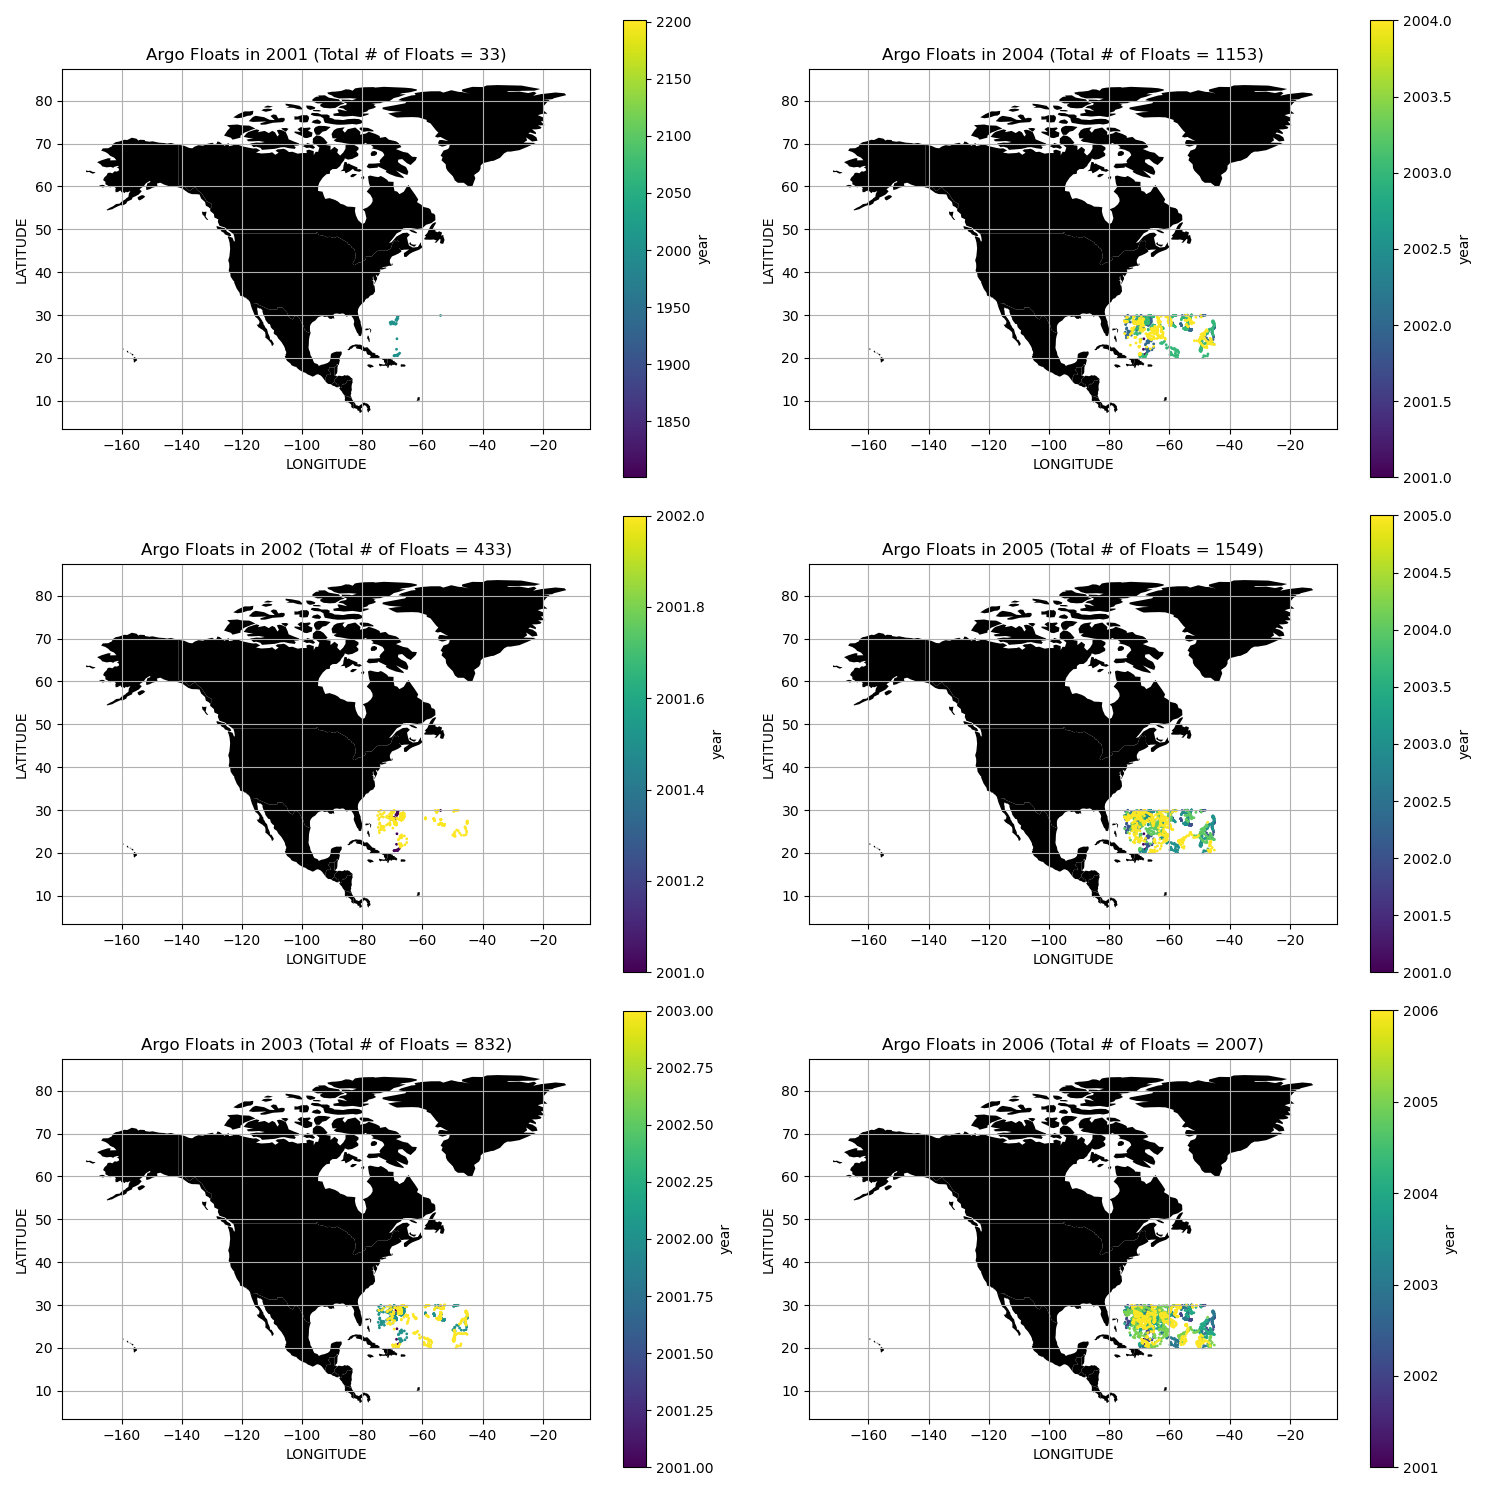
\includegraphics[width=\textwidth,height=\textheight,keepaspectratio]{total_argo.png}
 \caption{Total Argo floats for each year from 2001 to 2006 in a region southeast of Florida.}
 
\end{figure}

\subsection{Task 2 - Argo float trajectory and data}



\section{Conclusions}

\section{References}

Maze, G., & Balem, K. (2020). argopy: A Python library for Argo ocean data analysis. Journal of Open Source Software, 5(33).

\end{document}